\section{Experiments}
\label{sec:waveoptics:results}

In this section, we first validate our technique by comparing bulk scattering parameters computed with our method and the Lorenz-Mie theory (\S\ref{ssec:result_validation}).
Then, we apply our technique described in \S\ref{sec:waveoptics:ours_theory} and \S\ref{sec:waveoptics:ours_numerical} to compute bulk scattering parameters for a wide range of participating media (\S\ref{ssec:result_main}).


\subsection{Validation}
\label{ssec:result_validation}

To validate our technique, we compare computed bulk scattering parameters provided by our implementation and \texttt{MiePlot} \cite{laven2011mieplot}, a free software based on the Lorenz-Mie theory.
We focus on the configuration where a cluster contains only one (spherical) particle as this is a fundamental assumption of the Lorenz-Mie theory.

\begin{figure}[h]
    \centering
    \setlength{\resLen}{2.2in}
    \addtolength{\tabcolsep}{-6pt}
    \begin{tabular}{ccc}
        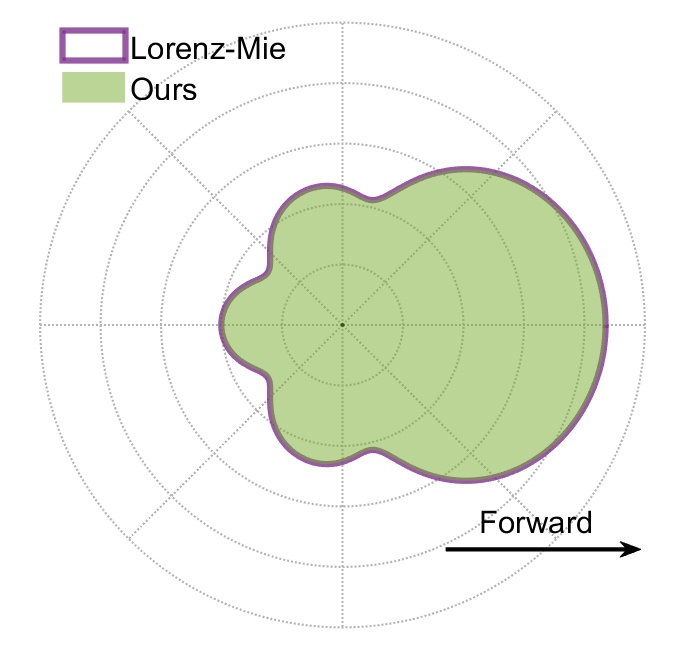
\includegraphics[width=\resLen]{waveoptics/pfunc/mie_300nm.jpg} & 
        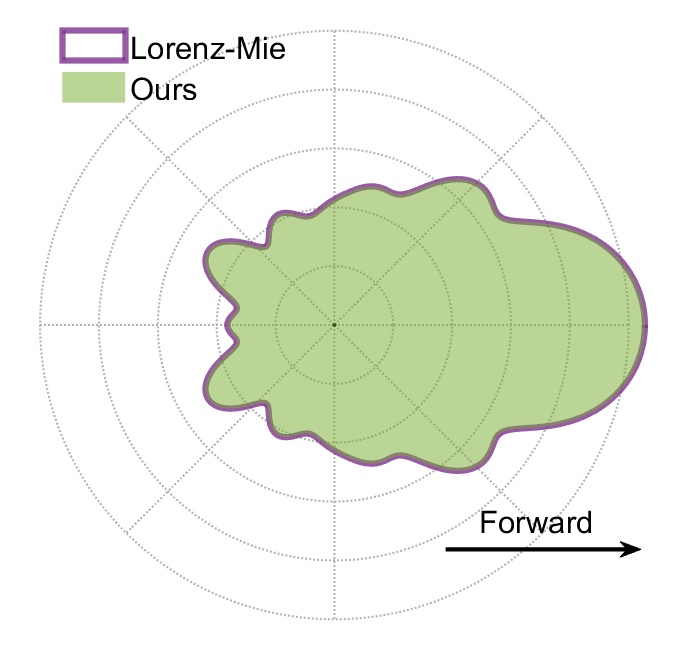
\includegraphics[width=\resLen]{waveoptics/pfunc/mie_600nm.jpg} &  
        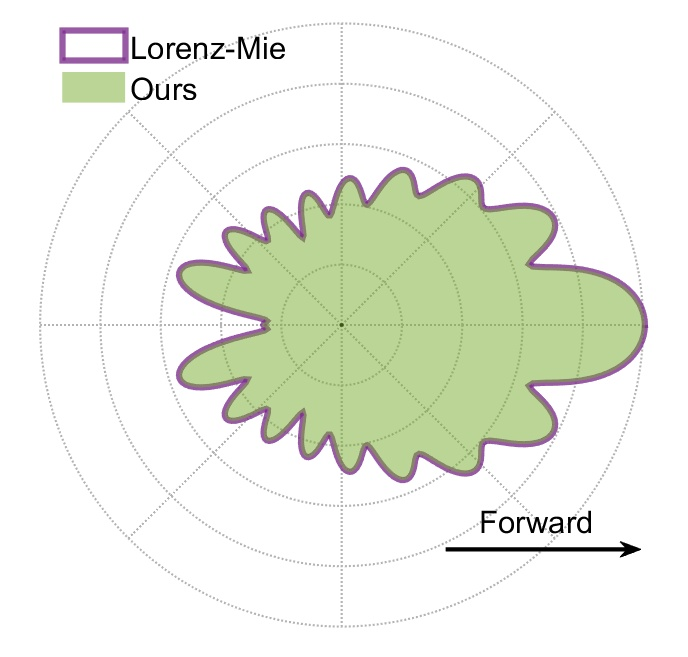
\includegraphics[width=\resLen]{waveoptics/pfunc/mie_900nm.jpg} 
        \\ 
        300nm & 600nm & 900nm
    \end{tabular}
    \caption[Comparison against Lorenz-Mie theory]{\label{fig:waveoptics:mie}
    	\textbf{Comparison against Lorenz-Mie theory.} We compare our method with clusters with a single particle $\Ncls=1$ against a reference solution based on Lorenz-Mie theory for three different particles radii~$a_i \in \{ \text{300nm, 600nm, 900nm} \}$. As expected, for a single particle our method reduces to the same results as Lorenz-Mie theory. The wavelength is $\lambda=600$nm, while the refractive index of the particle is $m=1.5+0.1\Img$.  
	}
\end{figure}


In Figure \ref{fig:waveoptics:mie}, we visualize computed single-scattering phase functions at the wavelength 600~nm with three particle radii (300, 600, and 900~nm).
We set the refractive index of the embedding medium to $(1.5 + 0.1\Img)$.

Additionally, we show in Figure \ref{fig:waveoptics:mie2} the corresponding extinction and scattering cross sections $\Ct$ and $\Cs$ given by Equations~\eqref{eq:crosstcluster} and \eqref{eq:crossscluster}, respectively.
In all these examples, our computed scattering parameters match those predicted by the Lorenz-Mie theory perfectly.

\begin{figure}[!ht]
    \centering
    \setlength{\resLen}{5in}
    \addtolength{\tabcolsep}{-3pt}
    \begin{tabular}{c}
        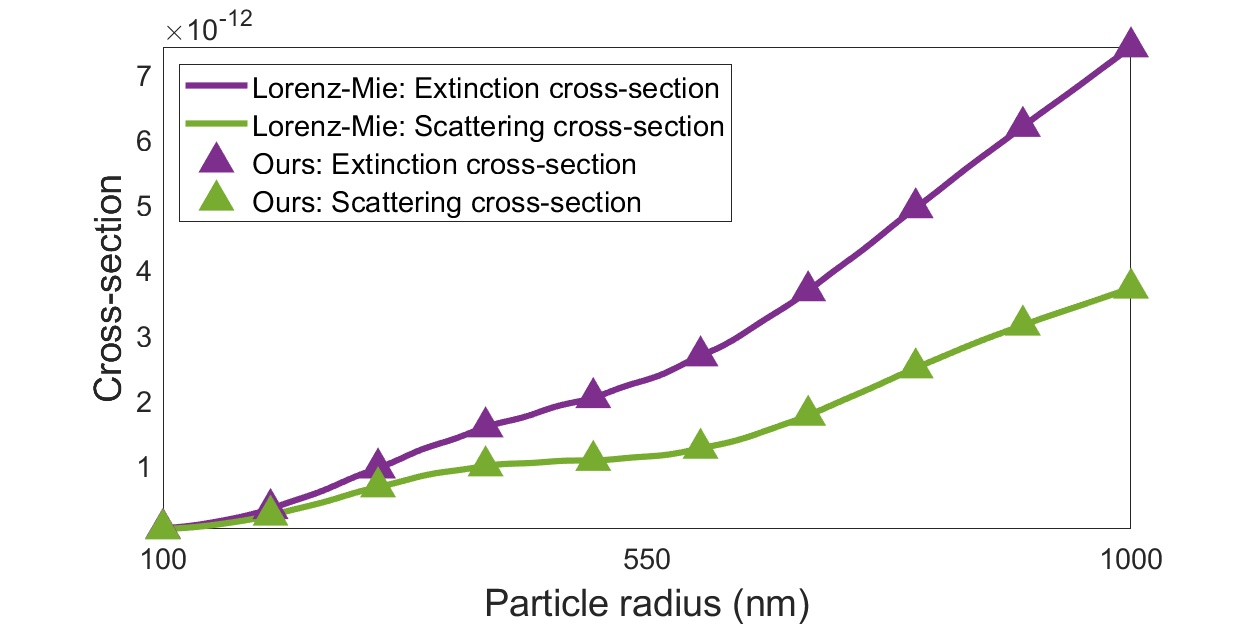
\includegraphics[width=\resLen]{waveoptics/pfunc/CsCt.jpg} 
    \end{tabular}
    \caption[Comparison against Lorenz-Mie theory 2]{\label{fig:waveoptics:mie2}
        \textbf{Comparison against Lorenz-Mie theory.} We compare the extinction and scattering cross sections computed with our method for $\Ncls=1$ against the results obtained using Lorenz-Mie theory. As in Figure \ref{fig:waveoptics:mie} our results show perfect agreement. 
	}
\end{figure}



\subsection{Main Results}
\label{ssec:result_main}
%
We now demonstrate the versatility of our technique by computing bulk scattering parameters for a range of participating media.
Please see Table~\ref{fig:waveoptics:time} for the performance statistics of our experiments.

\begin{table}[h]
	\centering
	\addtolength{\tabcolsep}{5pt}
    \caption[Performance statistics for our simulation]{\label{fig:waveoptics:time}
        \textbf{Performance statistics for our simulation.}
		The numbers are collected using a workstation equipped with an Intel i7-6800K six-core CPU and an Nvidia GTX 1080 GPU.
		To average the randomness of the particle position, we run 50 times for each simulation, so all the number should times 50 for the results in this chapter.
    }
    \begin{tabular}{cccc}
                                                               & N     & $\fp$ res.    & time   \\
    \hline
    Regular (Fig \ref{fig:waveoptics:lucycompare})             & 1-500 &  180x360         & 3-16s  \\
    Multi-spectral (Fig~\ref{fig:waveoptics:multiwave1})       & 100   &  180x360x50      & 35mins \\
    Anisotropic (Fig~\ref{fig:waveoptics:aniso2})              & 100   &  180x360x90      & 13mins \\
    Correlated (Fig~\ref{fig:waveoptics:correlated})           & 100   &  180x360         & 98s    \\
    \end{tabular}
\end{table}


\paragraph{Isotropic media}

In computer graphics, volumetric light transport effects are typically simulated using \emph{isotropic media} where the extinction and scattering coefficients $\sigmat$, $\sigmas$ are directionally independent, and the single-scattering phase function $\fp$ is formulated as a 1D function on the angle between the incident and scattered directions.

Our technique can produce bulk scattering parameters for isotropic media using particles distributed in radically symmetric densities.
We conduct a few ablation studies to demonstrate how different particle arrangements in a cluster affects the resulting parameters.
We use a wavelength of 600~nm for all these studies and represent the 1D phase functions as tabulated (i.e., piecewise constant) functions using 180 equal-sized bins.

\begin{figure}[!ht]
    \centering
    \setlength{\resLen}{2.1in}
    \addtolength{\tabcolsep}{-5.5pt}
    \small
    \begin{tabular}{ccc|ccc|ccc}
        \multicolumn{3}{c}{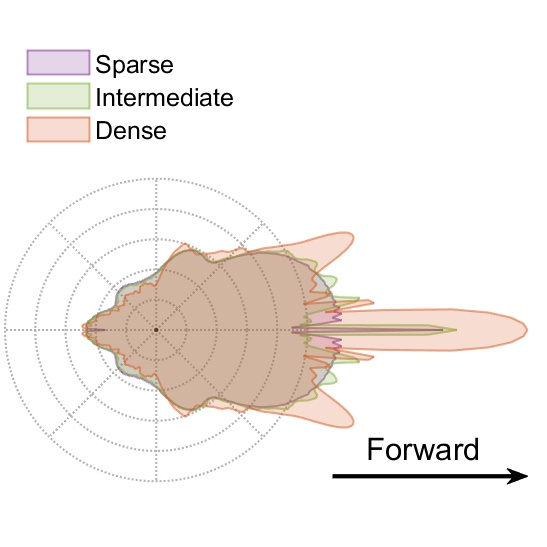
\includegraphics[width=\resLen]{waveoptics/pfunc/distance.jpg}} &
        \multicolumn{3}{c}{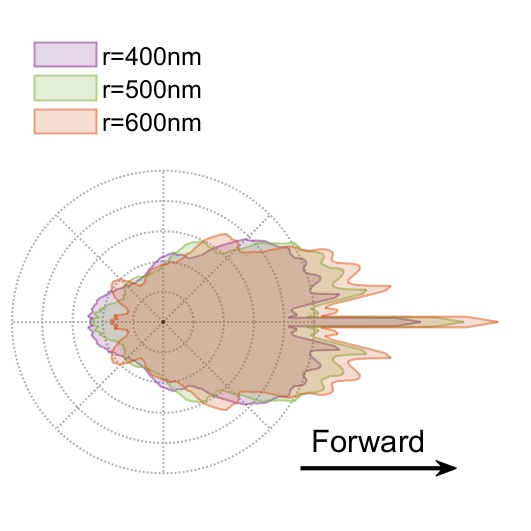
\includegraphics[width=\resLen]{waveoptics/pfunc/radius.jpg}} &
        \multicolumn{3}{c}{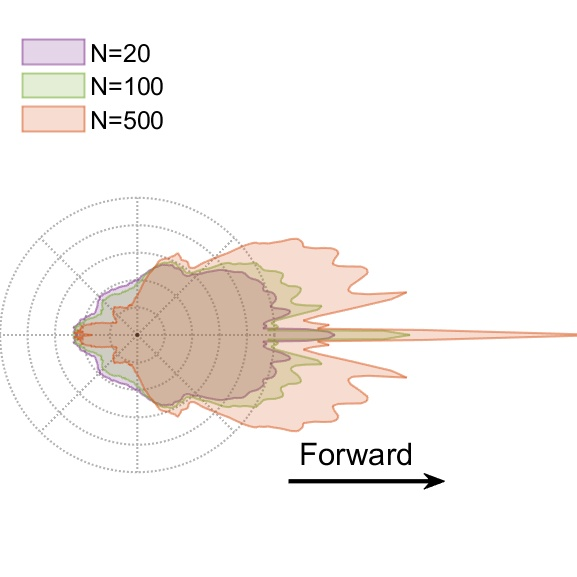
\includegraphics[width=\resLen]{waveoptics/pfunc/number.jpg}} \\[-5pt]
        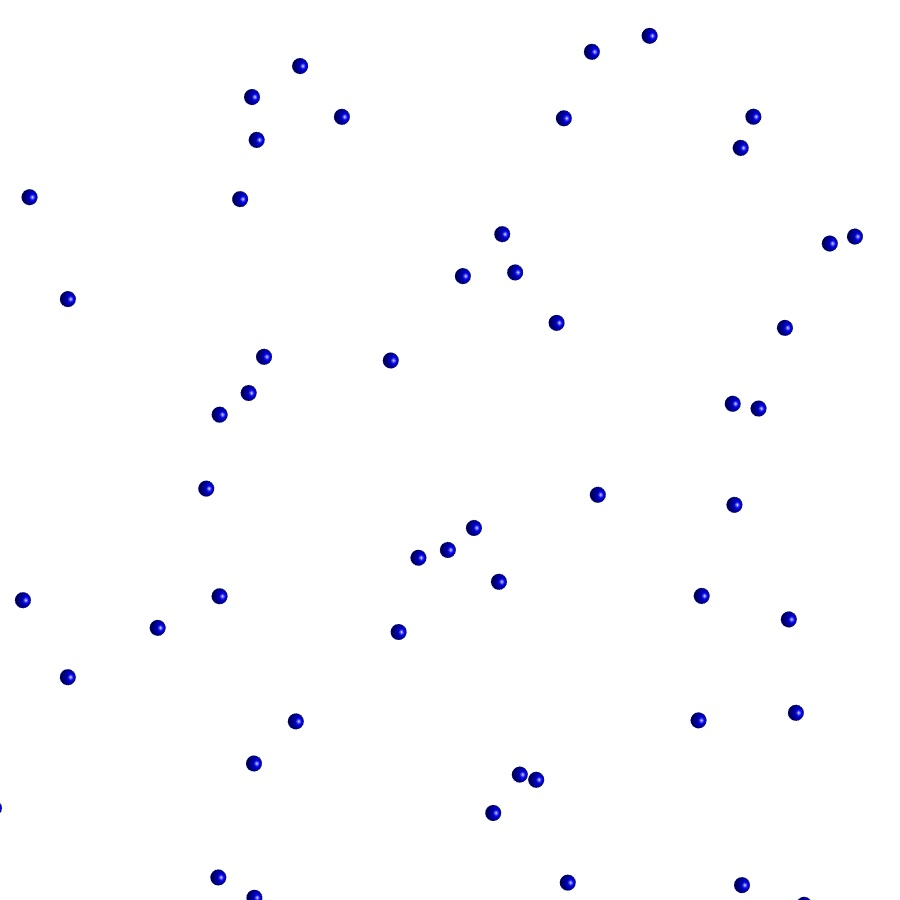
\includegraphics[width=0.33\resLen]{waveoptics/particle/validate2_D1_N100_500nm.jpg} &
        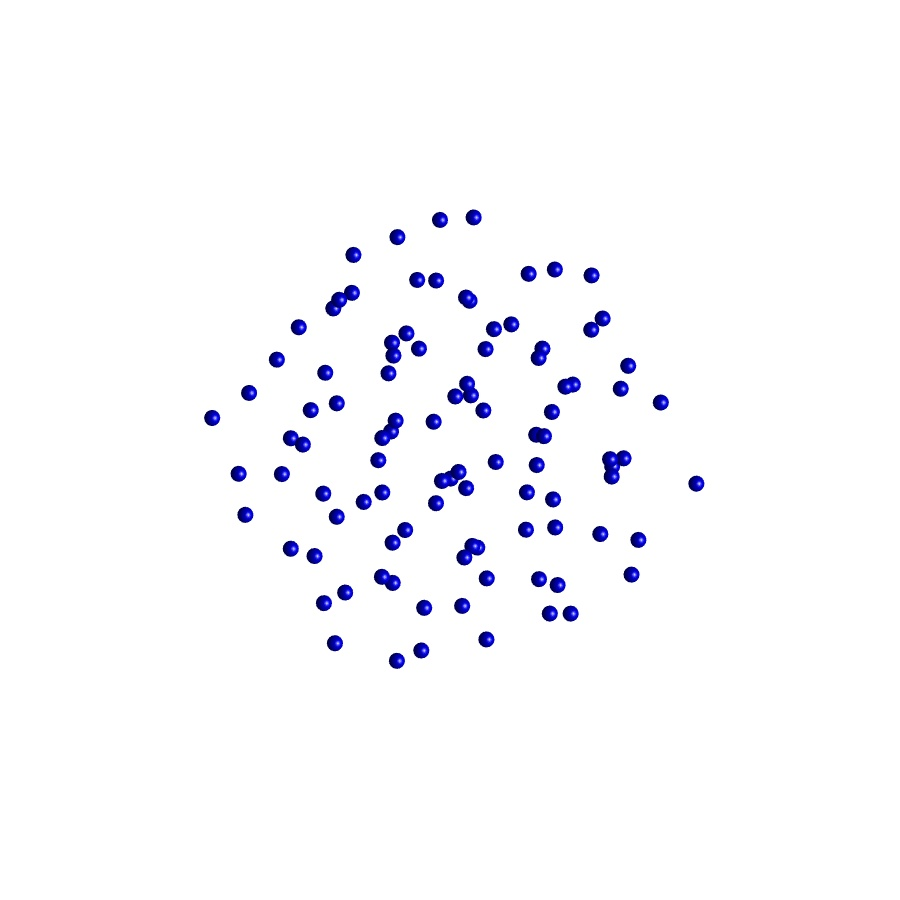
\includegraphics[width=0.33\resLen]{waveoptics/particle/validate3_D2_N100_500nm.jpg} &
        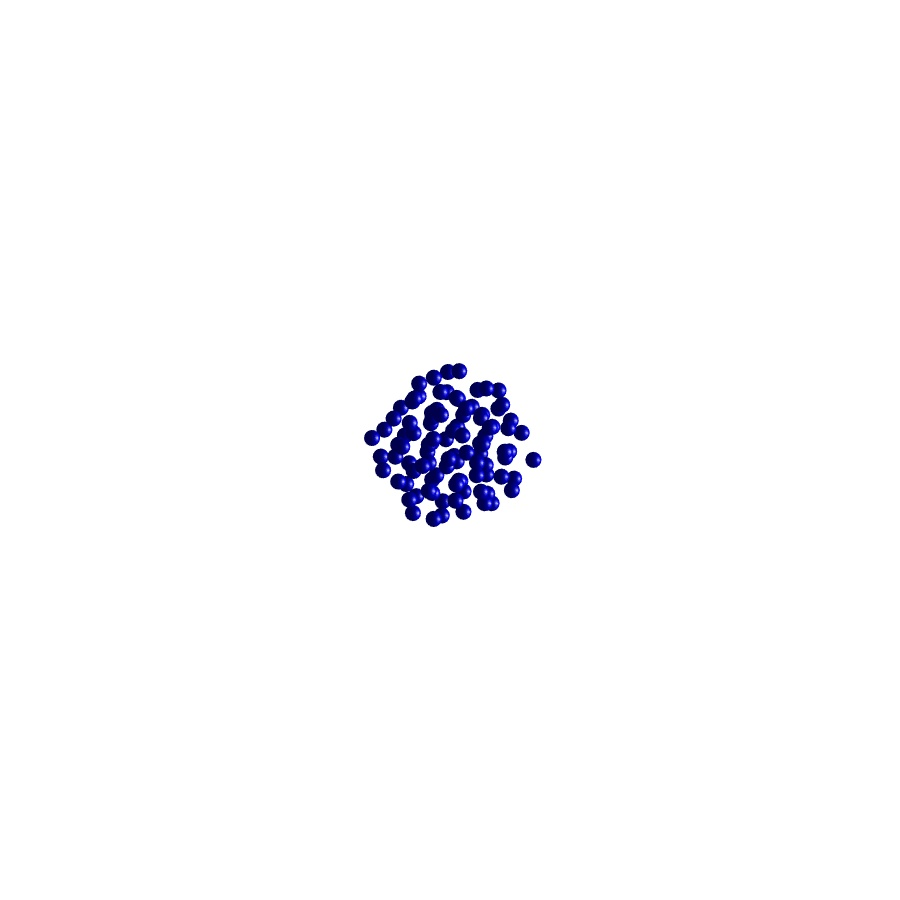
\includegraphics[width=0.33\resLen]{waveoptics/particle/validate4_D3_N100_500nm.jpg} &
        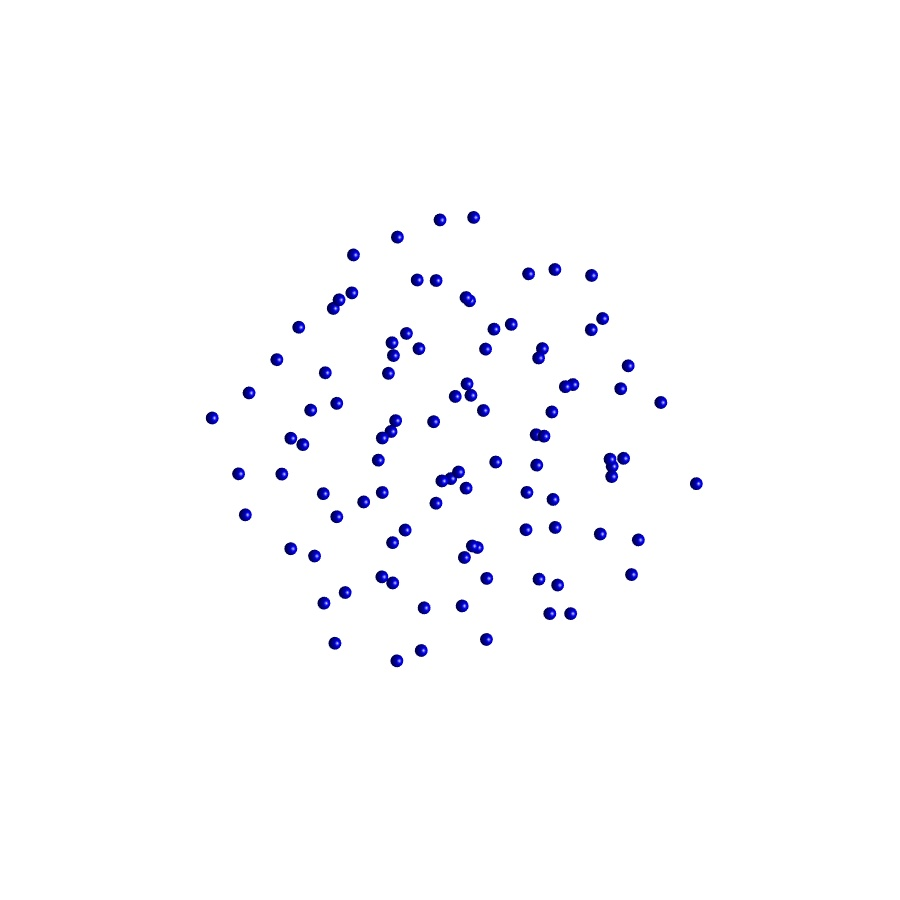
\includegraphics[width=0.33\resLen]{waveoptics/particle/validate5_D2_N100_400nm.jpg} &
        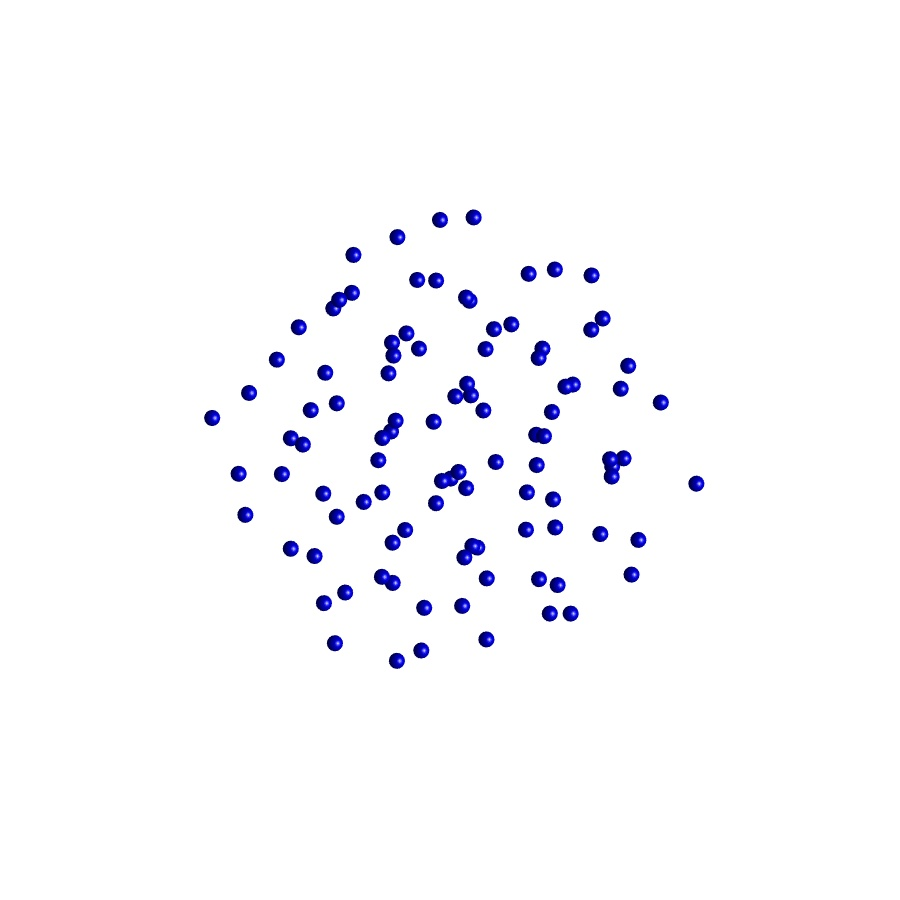
\includegraphics[width=0.33\resLen]{waveoptics/particle/validate3_D2_N100_500nm.jpg} &
        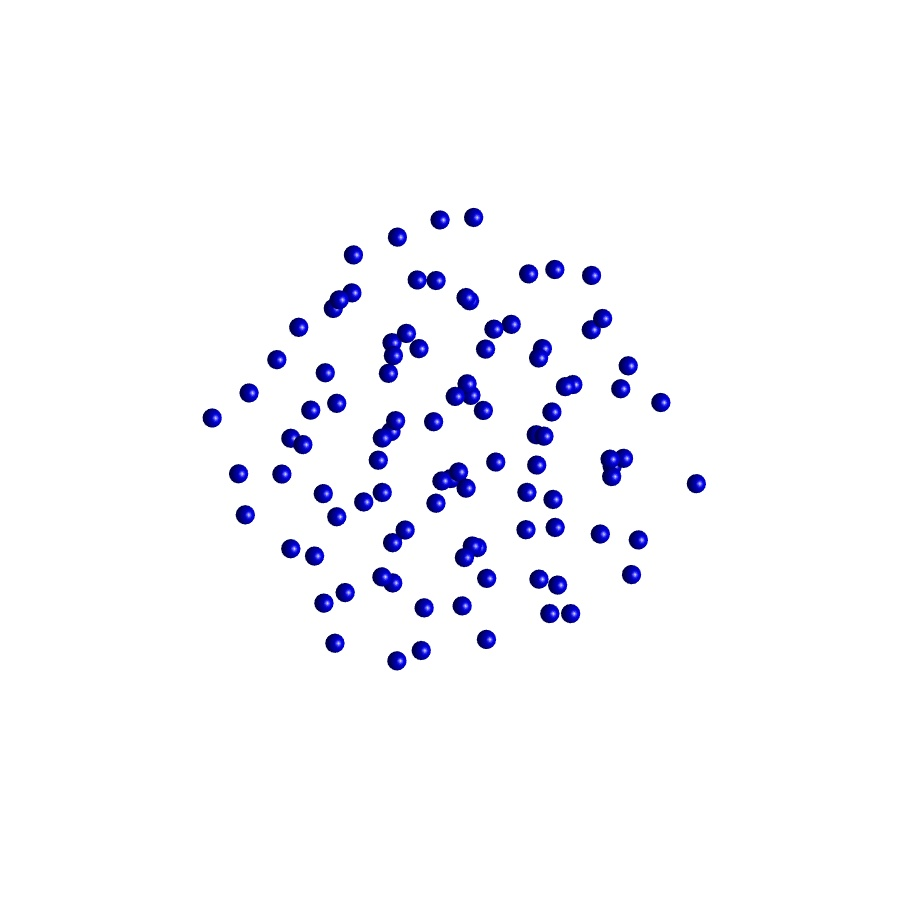
\includegraphics[width=0.33\resLen]{waveoptics/particle/validate7_D2_N100_600nm.jpg} &
        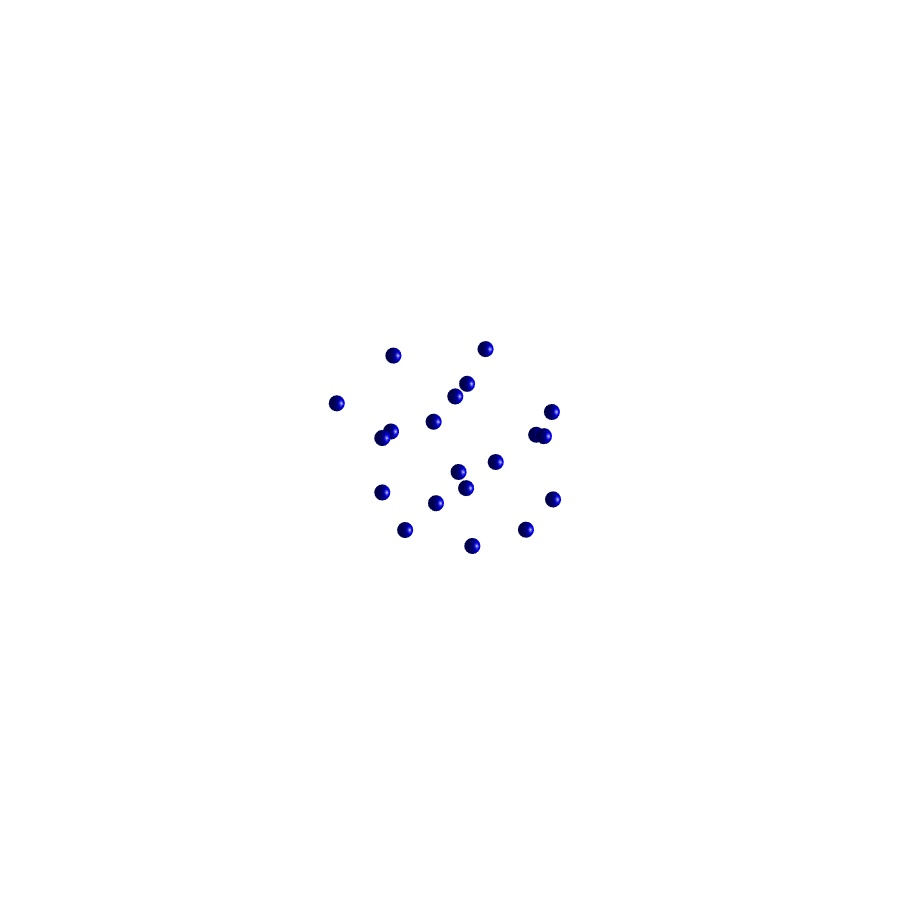
\includegraphics[width=0.33\resLen]{waveoptics/particle/validate8_D2_N20_500nm.jpg} &
        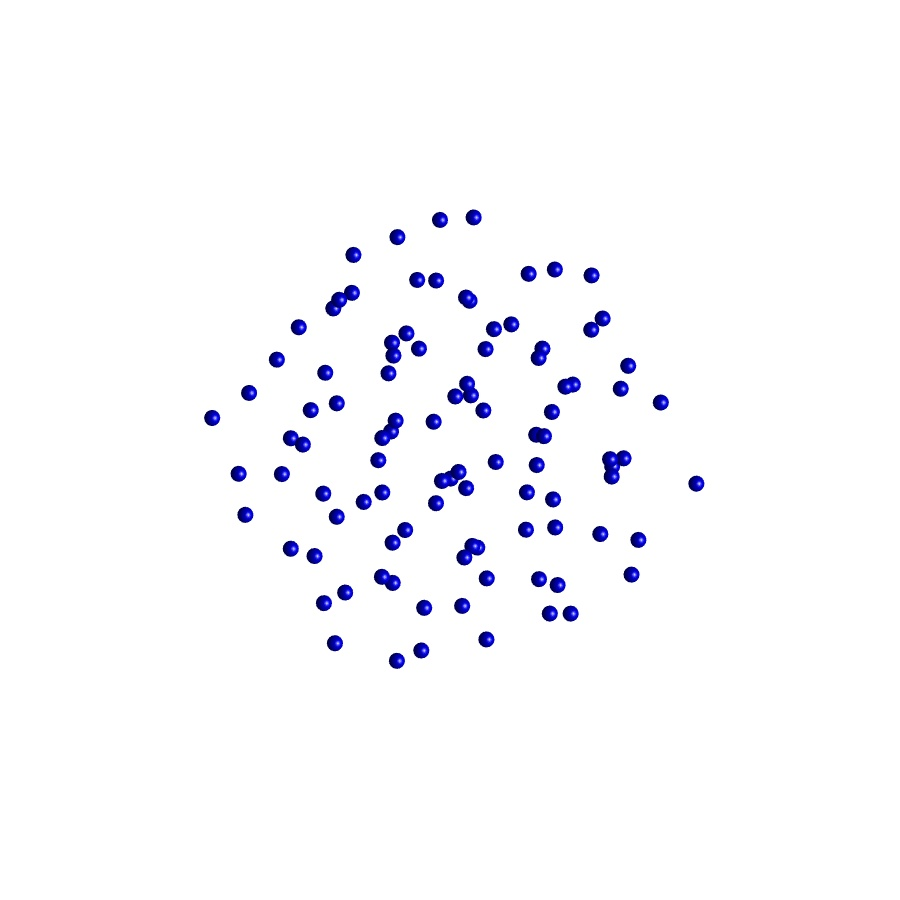
\includegraphics[width=0.33\resLen]{waveoptics/particle/validate3_D2_N100_500nm.jpg} &
        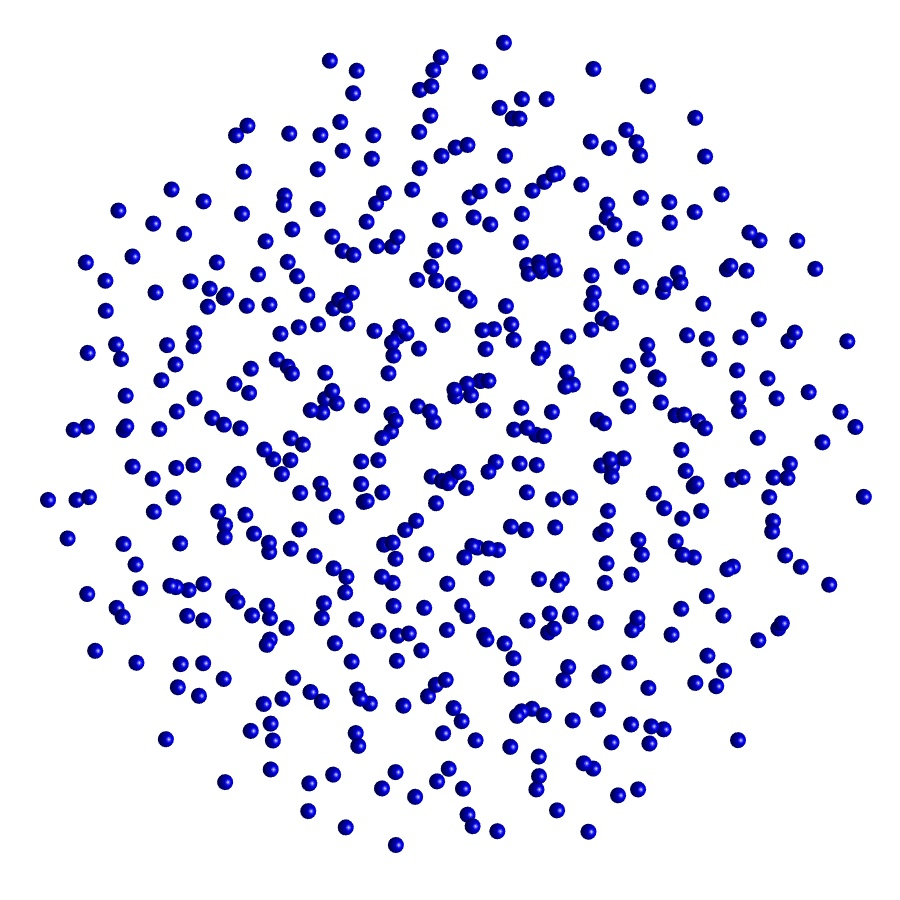
\includegraphics[width=0.33\resLen]{waveoptics/particle/validate10_D2_N500_500nm.jpg} 
        \\
        Sparse & Intermediate & Dense & $a_i$=400nm & 500nm & 600nm &
        $\Ncls=20$ & $100$ & $500$ \\ [5pt]
        \multicolumn{3}{c}{\textbf{(a)} Varying particles spacing} &
        \multicolumn{3}{c}{\textbf{(b)} Varying particles radius} &
        \multicolumn{3}{c}{\textbf{(c)} Varying particles count} 
    \end{tabular}
    \caption[Comparison for different parameters]{\label{fig:waveoptics:ablation}
        \textbf{Comparison of the resulting phase function} for different cluster parameters, for a planar incident field at $\lambda=700$nm. Unless mentioned otherwise, the clusters have $\Ncls=100$ particles, and each particle has radius $a_i=500$nm. For each phase function, we vary: (a) The distance between particles within the cluster; (b) The particle size $a_i$; and (c) The number of particles $\Ncls$. 
    }
\end{figure}

\begin{figure}[h!]
    \centering
    \setlength{\resLen}{2.55in}
    \setlength{\raiseLen}{1.3in}
    \addtolength{\tabcolsep}{-3.5pt}
    \begin{tabular}{ccccc}
		& $\Ncls=1$ & $\Ncls=50$ & $\Ncls=100$ & $\Ncls=500$
		\\
		\raisebox{\raiseLen}{\rotatebox[origin=c]{90}{$a_i=300\text{nm}$}} &
		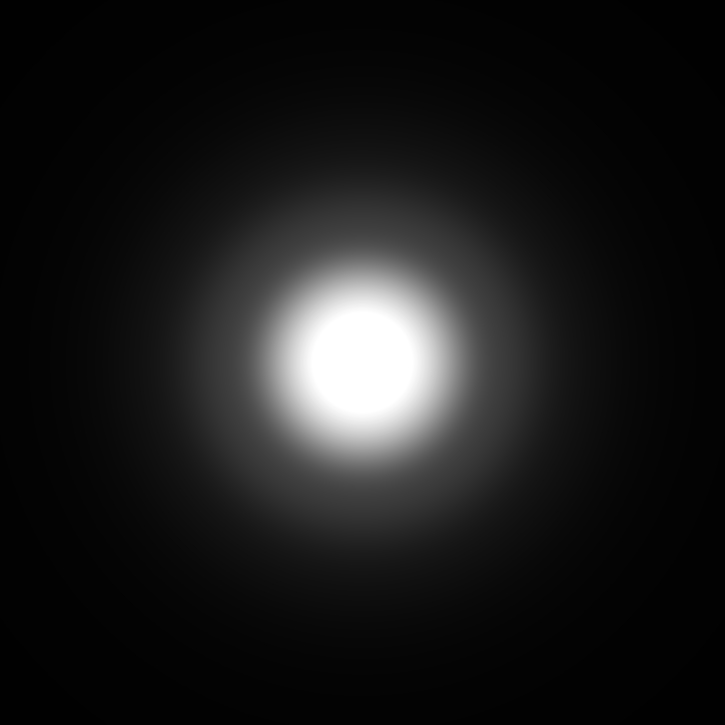
\includegraphics[height=\resLen]{waveoptics/lucy/N1_300nm.jpg} &
		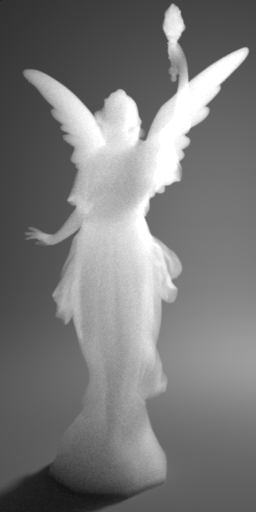
\includegraphics[height=\resLen]{waveoptics/lucy/N50_300nm.jpg} &
		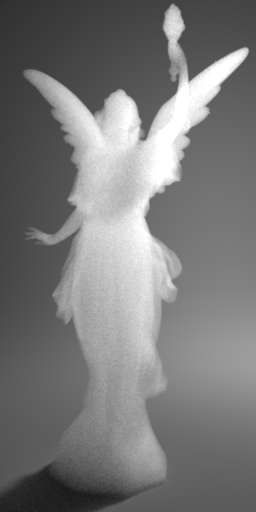
\includegraphics[height=\resLen]{waveoptics/lucy/N100_300nm.jpg} &
		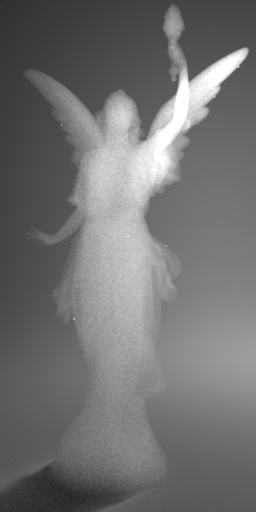
\includegraphics[height=\resLen]{waveoptics/lucy/N500_300nm.jpg}
		\\
		\raisebox{\raiseLen}{\rotatebox[origin=c]{90}{$a_i=400\text{nm}$}} &
		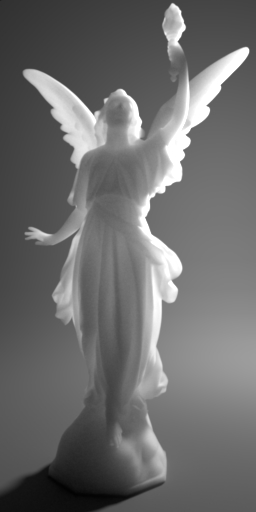
\includegraphics[height=\resLen]{waveoptics/lucy/N1_400nm.jpg} &
		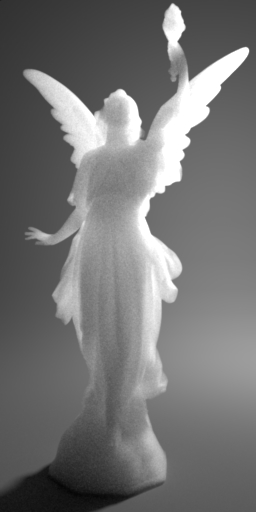
\includegraphics[height=\resLen]{waveoptics/lucy/N50_400nm.jpg} &
		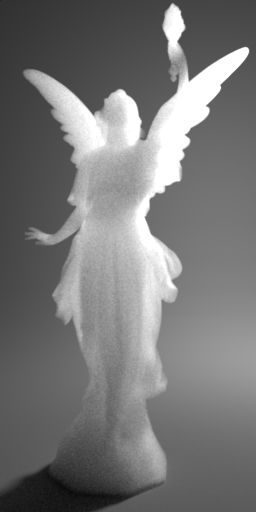
\includegraphics[height=\resLen]{waveoptics/lucy/N100_400nm.jpg} &
		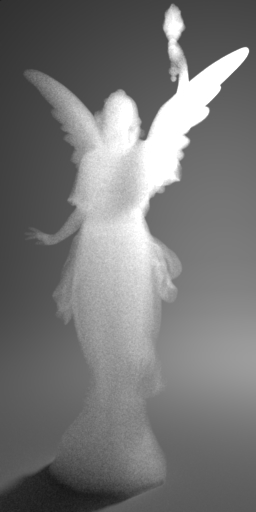
\includegraphics[height=\resLen]{waveoptics/lucy/N500_400nm.jpg}
		\\
		\raisebox{\raiseLen}{\rotatebox[origin=c]{90}{$a_i=500\text{nm}$}} &
		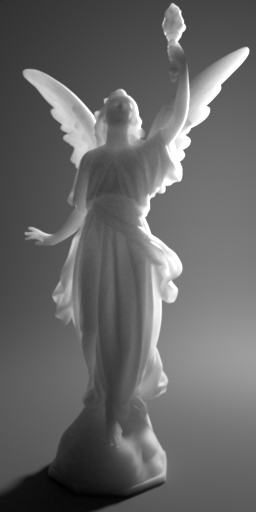
\includegraphics[height=\resLen]{waveoptics/lucy/N1_500nm.jpg} &
		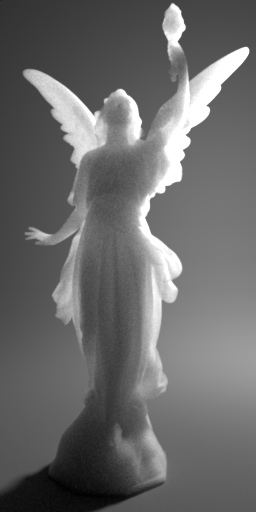
\includegraphics[height=\resLen]{waveoptics/lucy/N50_500nm.jpg} &
		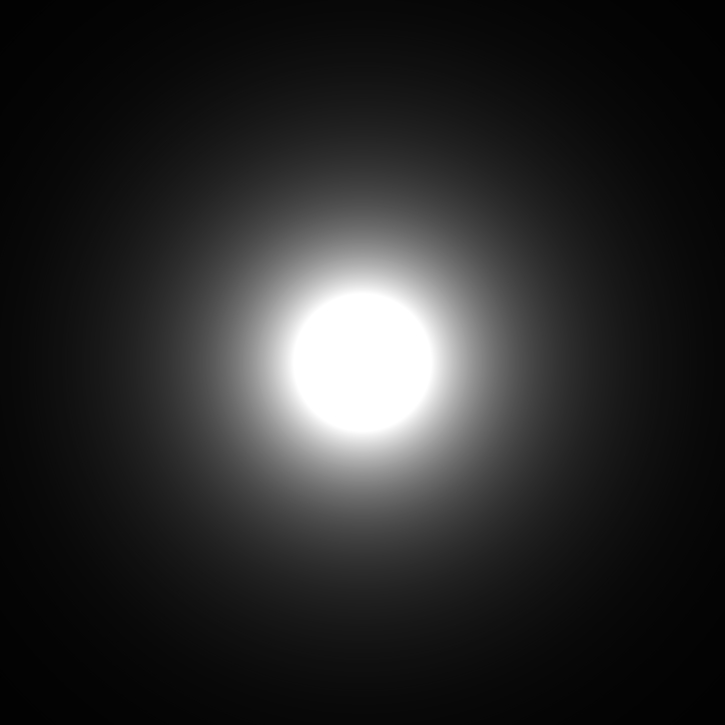
\includegraphics[height=\resLen]{waveoptics/lucy/N100_500nm.jpg} &
		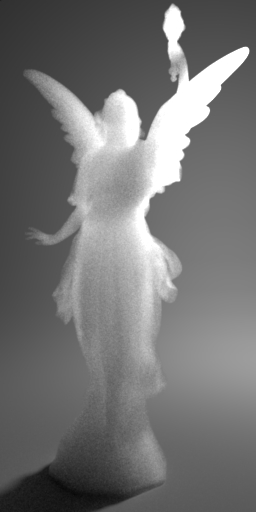
\includegraphics[height=\resLen]{waveoptics/lucy/N500_500nm.jpg} \\ [-10pt]
	\end{tabular}
    \caption[Renderings of homogeneous Lucy models]{\label{fig:waveoptics:lucycompare}
        \textbf{Renderings of homogeneous Lucy models} at $\lambda = 700\text{nm}$.
        The bulk scattering parameters are computed using our method with different combinations of particle radius $a_i$ and per-cluster particle count $\Ncls$.
    }
\end{figure}


In our first study, we use a cluster of 100 particles with radii 500~nm. Then, we vary the distances between particles (by using bounding spheres with different sizes and distributing particles uniformly in these spheres).
As shown in Figure \ref{fig:waveoptics:ablation} (a), the closer the particles are to each other, the more forward the resulting phase function is.
This is expected: With sparsely distributed particles, it is simpler for light to pass straightly through.

Our second ablation study examines the effect of particle size. With 100 uniformly distributed particles, we apply our technique to three particle sizes ($a_i$= 400, 500, and 600 nm).
As shown in Figure \ref{fig:waveoptics:ablation} (b), as we increase the particles radius, the phase function becomes more forward and increases its frequency. This agrees with the behaviour of single particles predicted by Lorenz-Mie theory. 

In our third study, we vary the number of particles in a cluster while keeping the particle size fixed to $a_i$=500 nm.
Figure \ref{fig:waveoptics:ablation} (c) shows that as we increase the number of particles, the phase function gets more forward and of higher-frequency, in a behaviour somewhat correlated with the particles size. This is the result of the increasing number of diffractive elements on the cluster, that instead of making scattering more diffuse (as predicted by geometric optics) increases its forward frequency. 

Lastly, we show in Figure \ref{fig:waveoptics:lucycompare} monochrome renderings using bulk scattering parameters obtained with varying combinations of particle count and radius.


\paragraph{Multi-spectral results}

Since our technique is derived using microphysical wave optics, it allows systematic generation of multi-spectral parameters based on a single (monochrome) configuration of particle cluster.

To demonstrate this, we use a configuration of 100 uniformly distributed particles (per cluster) with radius 500~nm and compute bulk scattering parameters at 50 wavelengths ranging from 400~nm to 700~nm.

\begin{figure}[h!]
    \centering
    \setlength{\resLen}{1.6in}
    \addtolength{\tabcolsep}{3pt}
    \begin{tabular}{cc}
        \begin{overpic}[height=\resLen]{waveoptics/pfunc/color.jpg}
            \put(2, 57){Ours}
        \end{overpic}
        &
        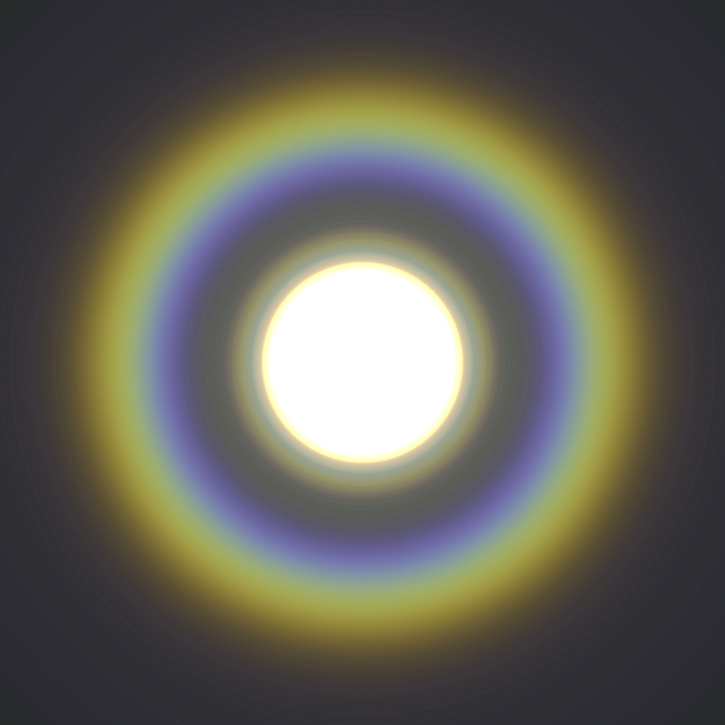
\includegraphics[height=\resLen]{waveoptics/slab/color4x.jpg}
        \\
        \begin{overpic}[height=\resLen]{waveoptics/pfunc/color1.jpg}
            \put(2, 57){Single-particle}
        \end{overpic}
        &
        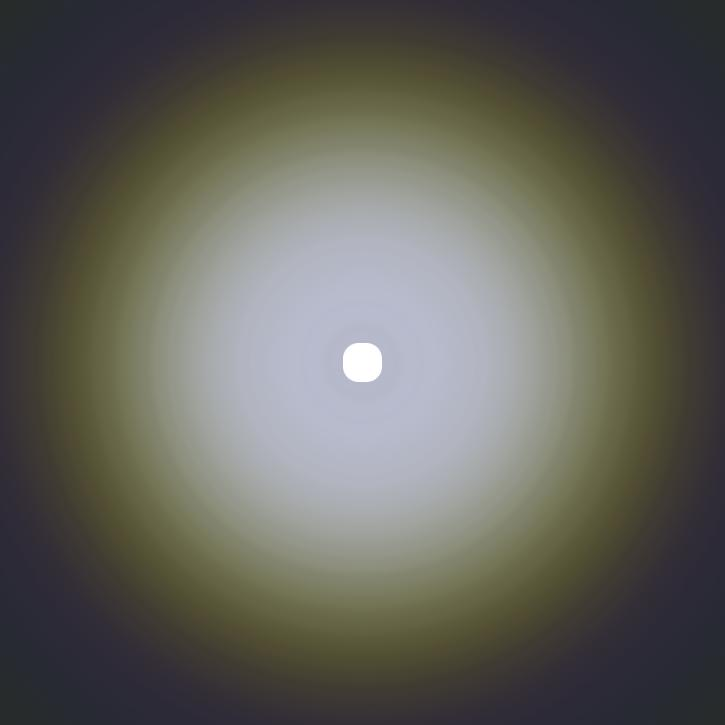
\includegraphics[height=\resLen]{waveoptics/slab/color4x_1.jpg}
        \\
        \textbf{(a)} Phase function & \textbf{(b)} Thin-slab rendering
    \end{tabular}
    \caption[Multi-spectral results]{\label{fig:waveoptics:multiwave1}
        \textbf{Multi-spectral results:} \textbf{(a)} visualizations of phase functions; \textbf{(b)} corresponding multi-spectral renderings of a thin slab lit by a small area light from behind.
        Results on the top are generated using a cluster of 100 particles with radii 500nm.
        Results on the bottom are obtained using a conventional single-particle setting.
        We used identical particle counts per differential volume for both configurations.
    }
\end{figure}


\begin{figure}[!ht]
    \centering
    \setlength{\resLen}{1.4in}
    \addtolength{\tabcolsep}{-3.5pt}
    %
    \begin{tabular}{cccc}
        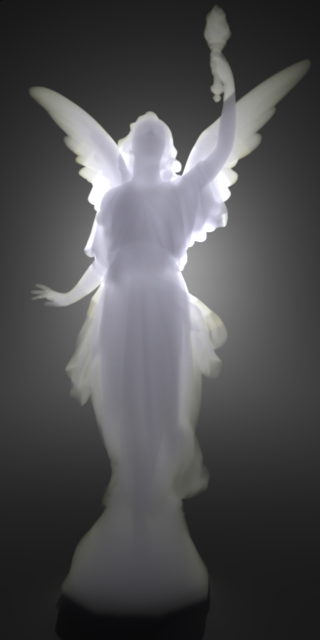
\includegraphics[width=\resLen]{waveoptics/lucy/color.jpg} &
        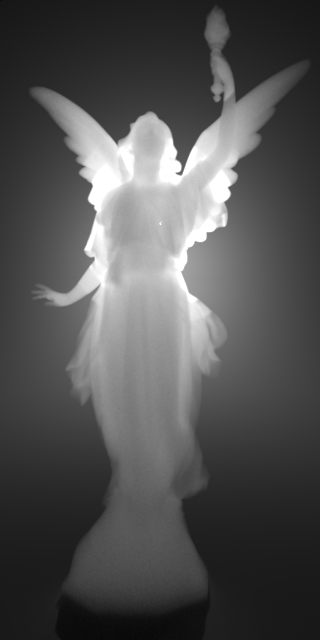
\includegraphics[width=\resLen]{waveoptics/lucy/color_400nm.jpg} &
        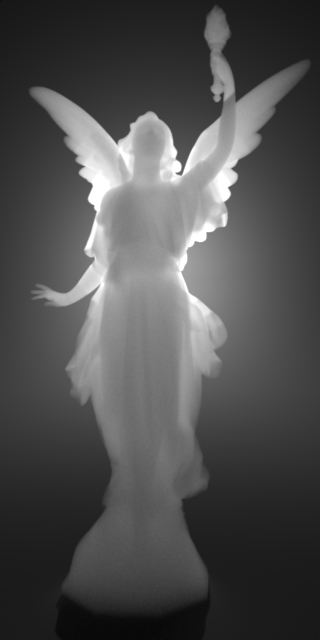
\includegraphics[width=\resLen]{waveoptics/lucy/color_550nm.jpg} &
        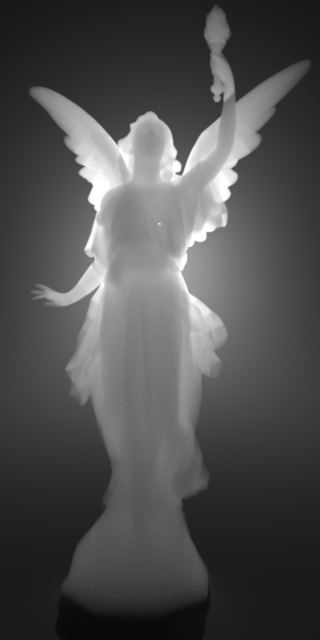
\includegraphics[width=\resLen]{waveoptics/lucy/color_700nm.jpg}
        \\
        \textbf{(a)} Multi. & \textbf{(b)} 400nm & \textbf{(c)} 550nm & \textbf{(d)} 700nm
    \end{tabular}
    \caption[Multi-spectral rendering of homogeneous Lucy model]{\label{fig:waveoptics:multiwave2}
        \textbf{Multi-spectral rendering of Lucy model.} \textbf{(a)} Multi-spectral rendering of a homogeneous Lucy model using identical bulk scattering parameters as the top row of Figure \ref{fig:waveoptics:multiwave1}.
        \textbf{(b--d)} Monochrome renderings of the same model at three wavelengths.
    }
\end{figure}


In Figure \ref{fig:waveoptics:multiwave1}, we visualize the computed phase functions at three wavelengths as well as multi-spectral renderings of a backlit thin slab.
The smooth changes in scattering parameters across wavelength have resulted in a characteristic rainbow-like effect.
When using the single-particle configuration (with identical overall particle density per unit volume), the rainbow effect is missing.

Figure \ref{fig:waveoptics:multiwave2} shows renderings of the Lucy model using these scattering parameters.


\paragraph{Anisotropic media}

Anisotropic media allow the extinction and scattering coefficients $\sigmat$, $\sigmas$ to be directionally dependent, and have full 4D phase functions $\fp$.
Previously, although the scattering parameters of anisotropic media can be devised based on the microflake models \cite{jakob2010radiative,heitz2015sggx}, equivalences of the Lorenz-Mie theory, to our knowledge, have been lacking. 

\begin{figure}[h]
    \centering
    \setlength{\resLen}{1.5in}
    \addtolength{\tabcolsep}{3pt}
    \begin{tabular}{ccc}
        & Forward & Backward\\
        \includegraphics[height=\resLen]{waveoptics/particle/aniso_z.jpg}
        & \multicolumn{2}{c}{\includegraphics[height=\resLen]{waveoptics/pfunc/aniso_z.jpg}}
        \\
        \includegraphics[height=\resLen]{waveoptics/particle/aniso_y.jpg}
        & \multicolumn{2}{c}{\includegraphics[height=\resLen]{waveoptics/pfunc/aniso_y.jpg}}
        \\
        \textbf{(a)} Incident direction & \multicolumn{2}{c}{\textbf{(b)} Phase function slice}
    \end{tabular}
    \caption[Visualizations of phase function]{\label{fig:waveoptics:aniso1}
        \textbf{Visualizations of slices $\fp(\hatbfni,\cdot)$ of a phase function} for two incident directions~$\hatbfni$ at $\lambda = 700\text{nm}$.
        This phase function is computed using a configuration where 100 particles with radii 500nm follow an anisotropic Gaussian distribution.
    }
\end{figure}


By using anisotropic particle distributions, our technique can generate bulk scattering parameters for anisotropic media.
To demonstrate this, we use a configuration where the cluster contains $\Ncls = 100$ particles following an anisotropic Gaussian distribution, as illustrated in Figure \ref{fig:waveoptics:aniso1}(a).
We tabulate the extinction and scattering cross sections using the latitude-longitude parameterization with a resolution of $180 \times 360$.
Due to the symmetry of the disc, the resulting phase function $\fp$ is three-dimensional, and we tabulated it with the resolution $90 \times 180 \times360$.

In Figure \ref{fig:waveoptics:aniso1}(b), we visualize slices of the computed single-scattering phase function $\fp$ with two incident directions $\hatbfni$.
In Figure \ref{fig:waveoptics:aniso2}, we show renderings of the Lucy model with three (spatially invariant) orientations.

\begin{figure}[!ht]
    \centering
    \setlength{\resLen}{1.4in}
    \addtolength{\tabcolsep}{-3.5pt}
    \begin{tabular}{ccc}
        \begin{overpic}[width=\resLen]{waveoptics/lucy/color_aniso_x_700nm.jpg}
            \put(2,2){\color{white} \textbf{700nm-x}}
        \end{overpic}
        &
        \begin{overpic}[width=\resLen]{waveoptics/lucy/color_aniso_y_700nm.jpg}
            \put(2,2){\color{white} \textbf{700nm-y}}
        \end{overpic}
        &
        \begin{overpic}[width=\resLen]{waveoptics/lucy/color_aniso_z_700nm.jpg}
            \put(2,2){\color{white} \textbf{700nm-z}}
        \end{overpic} \\
        \begin{overpic}[width=\resLen]{waveoptics/lucy/color_aniso_x.jpg}
			\put(2,2){\color{white} \textbf{Multi.-x}}
		\end{overpic}
		&
		\begin{overpic}[width=\resLen]{waveoptics/lucy/color_aniso_y.jpg}
			\put(2,2){\color{white} \textbf{Multi.-y}}
		\end{overpic}
		&
		\begin{overpic}[width=\resLen]{waveoptics/lucy/color_aniso_z.jpg}
			\put(2,2){\color{white} \textbf{Multi.-z}}
		\end{overpic}    
    \end{tabular}
    \caption[Renderings of homogeneous Lucy models]{\label{fig:waveoptics:aniso2}
        \textbf{Renderings of homogeneous Lucy models} with the same anisotropic medium as in Figure \ref{fig:waveoptics:aniso1}.
        With the medium's orientation -- which determines the axis of the disk -- aligned with the $x$-, $y$-, and $z$-axis, respectively, the Lucy model exhibit distinct appearances.
    }
\end{figure}



\paragraph{Correlated particles}

Finally, in Figure \ref{fig:waveoptics:correlated} we demonstrate the effect of particles correlation within the cluster, by analyzing particles distributed using both negative (Poisson sampled) and positive correlation \cite{jarabo2018radiative}. We compare the effect of introducing microscopic correlation on media where the clusters position is itself correlated, compared with uniformly distributed particles inside the clusters. These two levels of correlation have significant effect on the final appearance of the translucent materials. 

\begin{figure}[h!]
    \centering
    \setlength{\resLen}{1.45in}
    \addtolength{\tabcolsep}{-3.5pt}
    \begin{tabular}{cc|cc}
        \multicolumn{2}{c|}{\textbf{(a)} Negatively correlated particles} &
        \multicolumn{2}{c}{\textbf{(b)} Positively correlated particles}
        \\
        \multicolumn{2}{c|}{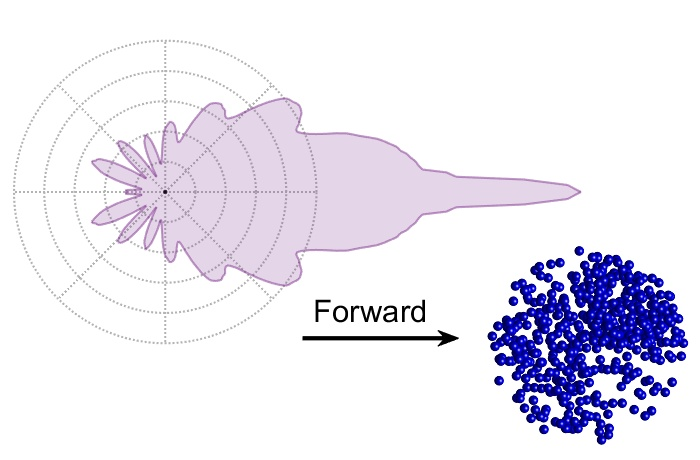
\includegraphics[width=2\resLen]{waveoptics/pfunc/neg_merge.jpg}} & \multicolumn{2}{c}{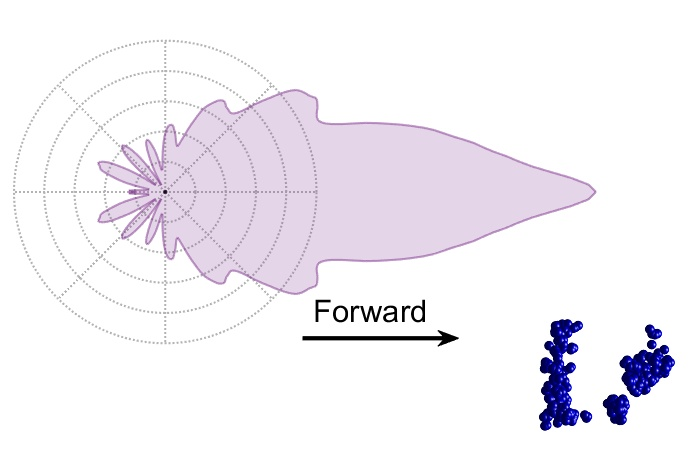
\includegraphics[width=2\resLen]{waveoptics/pfunc/pos_merge.jpg}} 
        \\
        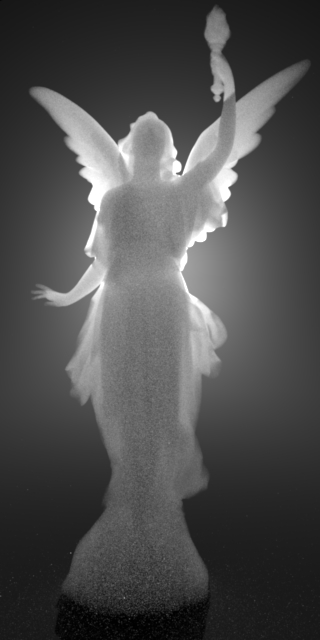
\includegraphics[width=\resLen]{waveoptics/lucy/neg_unc.jpg} &
        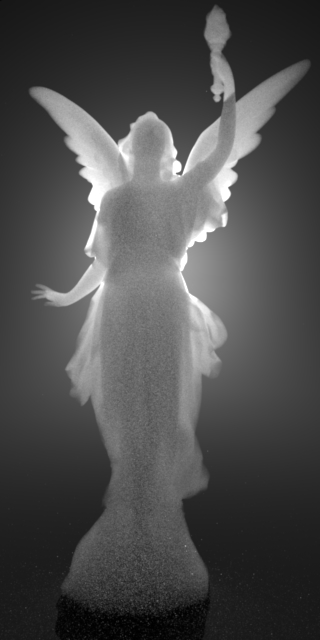
\includegraphics[width=\resLen]{waveoptics/lucy/neg_neg.jpg} &
        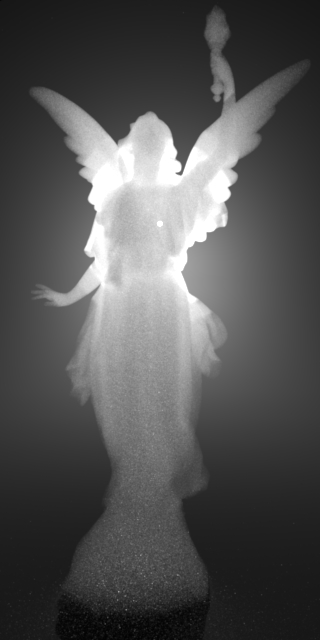
\includegraphics[width=\resLen]{waveoptics/lucy/pos_unc.jpg} &
        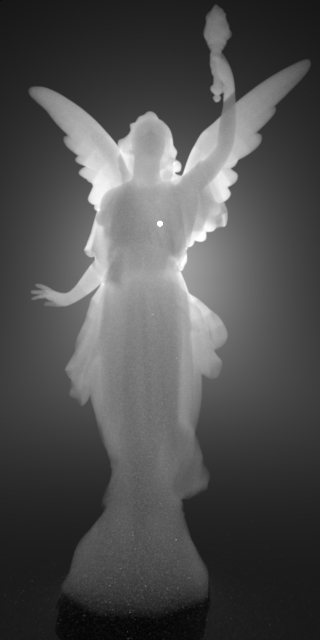
\includegraphics[width=\resLen]{waveoptics/lucy/pos_pos.jpg} 
        \\
        \textbf{(a1)} unc. clusters & \textbf{(a2)} neg. clusters & \textbf{(b1)} unc. clusters & \textbf{(b2)} pos. clusters
    \end{tabular}
    \caption[Correlated particles]{\label{fig:waveoptics:correlated}
        \textbf{Correlated particles:} By correlating particle positions in negatively (a) or positively (b), our method can produce bulk scattering parameters for correlated media.
        In this example, we use $\lambda = 400\text{nm}$, particle radius $a_i = 500\text{nm}$, and per-cluster particle count $\Ncls = 100$.
        Additionally, we can further correlate particle clusters themselves, a variety of appearances can be achieved (\textbf{a1--b2}).
        (The bright dot in \textbf{(b1)} and \textbf{(b2)} emerges from unscattered light from the area source.)
    }
\end{figure}


